\chapter{Literature review}
\section{Important issues in comparative simulation studies}

\noindent \parencite{polce_guide_2023} Show that the literature on ML in orthopedics is predominantly composed of preliminary studies, and frequently lacks depth in addressing complex ML concepts and often falls short in providing comprehensive method specification for result interpretation. \parencite{polce_guide_2023} Continues to explain that deep Learning is a prominent subset of ML, and utilizes neural networks to process both structured and unstructured data, enhancing the capability to handle diverse data types like images and texts. Similarly \parencite{smith_scoping_2022} show out of their methodical study selection process that only a handful of studies have attempted such comparisons at an acceptable standard, while most studies focus predominantly on machine learning techniques neglecting the broader spectrum of statistical methods. 
\\\\
Furthermore \parencite{smith_scoping_2022} point out authors often omit interaction terms and non-linear covariate effects which are essential components for enhancing model robustness and accuracy. The predominance of studies failed to relax the proportional hazards assumption which underscores a critical oversight in adapting models to more complex datasets. Finally and more broadly \parencite{smith_scoping_2022} show that there is a need for comprehensive methodological improvements and enhanced reporting standards to ensure reproducibility and a fair assessment of method capabilities.
\\\\
Common issues include inadequate design and reporting that lead to uncritical acceptance of results. This lack of rigor can result in misleading conclusions, for example, the variability introduced by different sets of random numbers in Monte Carlo simulations that are sometimes ignored. \parencite{smith_scoping_2022} Found a notable scarcity of quality comparative research between statistical and machine learning methods. Predominantly, these studies focus on machine learning techniques while traditional statistical methods are often neglected. For instance, it was common for some authors to overlook the inclusion of interaction terms and non-linear covariate effects in the Cox model as well as time-dependent effects which are key elements for effectively handling complex datasets. The reporting standards of the reviewed studies were also generally poor. Important details such as data-generating mechanisms (DGMs), estimands, and method implementations are frequently underreported, which impedes the reproducibility of the research and the ability to conduct fair comparisons between methods. \parencite{smith_scoping_2022} also pointed out that a significant bias could be observed in the selection of DGMs, which tend to favor machine-learning approaches, especially in scenarios where the number of variables exceeds the sample size. This predisposition can lead to biased results unless the study incorporates specific statistical variable selection techniques that are suited for high-dimensional data. Additionally, the prevalent use of the C-index as the sole performance metric, without accounting for calibration is noted. By relying solely on this metric results analysis may not provide a complete picture of the model's predictive accuracy over time, particularly when the proportional hazards assumption is not valid.
\\\\
Finally, \parencite{smith_scoping_2022} exclaim that there is a concerning lack of expertise in implementing complex statistical methods thoroughly. This deficiency often results in potentially misleading outcomes that do not genuinely reflect the true performance capabilities of the methods being compared. The findings underscore the need for improved methodological rigor and enhanced collaboration among researchers to ensure that both statistical and machine learning methods are implemented to their full potential and evaluated fairly. As a framework \parencite{pawel_pitfalls_2024} formalizes the use of indicators, defined as “questionable research practices” (QRP) which indicate faulty research methods used widely throughout simulation studies, which should get the necessary attention. The QRP's are categorized during phases of comparative simulation, namely the design phase, execution phase, and reporting phase this is shown in Figure \ref{fig:qrp}. \parencite{pawel_pitfalls_2024} Labels specific components of simulation studies, an example being D1 which references “the data-generating process”, and cross correlates with other components to define QRP occurrence and relationships.


\section{Models}
\subsection{Cox's Proportional Hazards Model}

\noindent In the seminal work by \parencite{cox_regression_1972}, the Cox model is introduced as an extension to prior work formalized as the Kaplan-Meier estimator, by exploring time-to-event data (life tables). The major benefit is that it addresses censored data, which is a known concept in survival analysis, that there is missing information within the data, specifically, event occurrence without observation on a continuous time scale. Hazard is the estimated conditional probabilities, in line with the observed conditional frequencies of events or simply the risk of event occurrence at a specific time.
\\\\
\textit{Time-Dependant Covariates}
\par \noindent The Cox model incorporates both time-independent and time-dependent covariates. \parencite{kalbfleisch_fifty_2023} Time-dependent covariates can change over the time, such as \(Z_{2}(t) = Z_{1}t^{*}\). This flexibility allows the model to handle scenarios where hazards are not proportional, which extends its applicability. Relative risk is represented as \(\exp{Z(t)'}\), showing how risk changes with time and covariate values, and depending on the coefficients, the relative risk in a treatment group can increase, decrease, or remain constant over time. \parencite{kalbfleisch_fifty_2023} External covariates are variables that are independent of the subject's survival process. Whereas internal covariates are variables that might influence and be influenced by survival. \parencite{kalbfleisch_fifty_2023} Different approaches for modeling survivor functions are required for external and internal covariates due to their nature.
\\\\
\noindent \parencite{woo_time_2023} Proposes a step-by-step development and testing of time dependence in the Cox model, with emphasis on methods and critical formulas to highlight key concepts in understanding and applying time-dependent effects in survival analysis. \parencite{woo_time_2023} Point out how the impact of variables can change over time, which is critical for understanding complex dynamics in data that cannot be captured by static models. Step 1 includes the selection and justification of the appropriate survival time variable for use in the Cox model. Accurate identification of the "at risk" period is crucial for defining when subjects are susceptible to the event of interest. The measurement scale (e.g., years, and months) should match the scale of independent variables. It is noted about 50\% of the reviewed studies properly justified their choice of survival time variable, highlighting the need for a clear explanation. Step 2 is for developing time-dependent moderation hypotheses based on a priori theory-building. It is a good indication of the importance of time dependence as it directly shows effects between \parencite{woo_time_2023} the three types of time-dependent effects are type 1; both main and moderation effects are significant and in the same direction, thereby strengthening each other. Type 2; main and moderation effects are significant but in opposite directions, thereby weakening the main effect. Type 3; only the moderation effect is significant with no main effect, showing causality only in extended survival times. Step 3, tests for the proportional hazards assumption, using graphical methods like log-log survival curves. \parencite{woo_time_2023} This however is subjective and lacks statistical tests, problematic with continuous variables. Another approach is to approximate goodness-of-fit by using the Schoenfeld residuals test, which can detect non-zero slopes in survival time against scaled Schoenfeld residuals to check PH assumption violations. Step 4: Shows the extended Cox Model by integrating time-dependence detected from PH tests and adding interaction terms to the model. Interaction terms are the product of time and independent variables to handle non-proportional hazards. The extended Cox model equation: \(h(t,X) = h_{0}(t).\exp{b_{1}x+b_{2}xt+b_{3}z}\). Lastly, Step 5 is to interpret the effects of the time dependence integration by computing hazard ratios over time to understand changes in effects due to survival time, using the extended model. \parencite{woo_time_2023} This allows the use of model results to further develop or adjust theoretical assumptions based on observed data. Hazard Ratio calculation for time-dependence, \(\hat{HR} = \exp{b_{1}+b_{2}t}\)
\\\\
\textit{Likelihood Function}
\par \noindent The various approaches to the Cox model handle data ties and time-dependent covariates differently, \parencite{kalbfleisch_fifty_2023} recommended specific methods based on the data structure (e.g., number of ties). The concept of partial likelihood is particularly important as it provides a way to focus on relevant factors in the presence of complex data types, enhancing both the theoretical understanding and practical application of the Cox model. The marginal likelihood approach \parencite{kalbfleisch_fifty_2023} (Kalbfleisch \& Prentice, 1973), was developed for both uncensored and censored data. In uncensored scenarios, it treats the ranks of data points as arising from the marginal distribution, leading to the Cox likelihood. It allows for a statistical handling of tied data points by breaking ties in all possible ways, which though accurate, is computationally intensive. \parencite{kalbfleisch_fifty_2023} Breslow's step function approach (1974), assumes a step function for the baseline hazard with changes at observed failure times. Simplifies computations but is less theoretically satisfying as the model depends on the data itself. This approach is particularly useful for handling time-dependent covariates. \parencite{kalbfleisch_fifty_2023} Bailey's non-parametric approach (1984), which uses a nonparametric maximization of the full likelihood. This provides estimators for regression coefficients and survival probabilities similar to those in previous methods. Finally the partial likelihood \parencite{kalbfleisch_fifty_2023} (Cox, 1975), uses partial likelihood for estimation, separating the effect of nuisance parameters. This approach simplifies the computational process and can isolate useful data from noise.
\\\\
% \noindent The survivor function used calculates the probability of surviving (not failing) past time \(t\) considering all causes.

% \begin{equation} \label{eq:spesificsurvivor}S(t|Z) = \exp(-\int_{0}^{t} h(u|Z) du)\end{equation}

% \noindent Cumulative Incidence Function is shown to be the probability of failing from cause \(j\) by time \(t\), accounting for competing risks.

% \begin{equation} \label{eq:cumulativeincidence}F_{j}(t|Z) = \int_{0}^{t} h_{j}(u|Z)S(u|Z)du\end{equation}

% \noindent The subdistribution hazard \parencite{kalbfleisch_fifty_2023}(Fine \& Gray Model), specifically focuses on the hazard of a particular cause while considering other causes as competing events, by directly modeling the cumulative probability of the event of interest.

% \begin{equation} \label{eq:subdistribution}\tilde{a}_{j}(t|Z) = \frac{d}{dt}log(1-F_{j}(t|Z))\end{equation}

\subsection{Lasso Regularisation For Variable Selection }
\noindent By penalizing the sum of the absolute values of the model parameters, the LASSO method encourages models with fewer parameters. This can lead to the exclusion of some variables entirely if their effect is not strong enough to justify a larger coefficient size given the regularisation penalty. LASSO can incorrectly include or exclude important variables, known as false discoveries. Enhanced methods like Adaptive LASSO, and Stability Selection are used to improve variable selection accuracy. The choice of \(\lambda\) affects the sparsity of the resulting model; too large a \(\lambda\) might shrink all coefficients to zero. The \(\lambda\) parameter is often chosen via cross-validation by optimizing some criterion (e.g., AIC, BIC, MSE). \parencite{freijeirogonzalez_critical_2022} Popular extensions of the lasso method includeded in Table \ref{tab:methlasso}.

\begin{table}
\begin{tabularx}{\textwidth}{|X|X|X|}
    \hline
    Method & Library & Description \\
    \hline
    LASSO & glmnet & Regularized regression encourage sparse solutions by adding a penalty proportional to the absolute value of the coefficients. \\
    \hline
    SCAD & ncvreg & Non-convex penalty that encourages sparsity without overly penalizing large coefficients, more continuity in coefficient estimation compared to Lasso \\
    \hline
    Adaptive Lasso & adapl \& glmnet & weights penalties based on initial estimates to improve consistency. \\
    \hline
    Dantzig Selector & Dant \& flare & Ensures residuals are small and the solution is sparse, focussing on covariate selection accuracy \\
    \hline
    Relaxed Lasso & relaxl \& relaxo & Combines Lasso solution with unpenalized least squares, reducing bias and variability  \\
    \hline
    Square-root Lasso & sqrtl \& flare & Modification of lasso stabilizing noise level variability \\
    \hline
    Scaled Lasso & Scail \& scalreg & Adjusts the penalty term dynamically based on residual variance, improving error rate and variable selection \\
    \hline
\end{tabularx}
\caption{Libraries illustrating Lasso implementations. \parencite{freijeirogonzalez_critical_2022}}
\label{tab:methlasso}
\end{table}
\pagebreak
\noindent \textit{Adaptive Lasso}
\\
\noindent By using weights that are inversely proportional to the magnitude of initial estimates, \parencite{zhang_adaptive_2007} Adaptive Lasso can differentiate more effectively between relevant and irrelevant predictors, for variable selection. Regularisation helps prevent overfitting, a common issue in models trained on high-dimensional data. \parencite{zhang_adaptive_2007} By penalizing the sum of the absolute values of the coefficients, the Adaptive Lasso ensures that the model generalizes well to unseen data. Compared to the standard Lasso, the adaptive version reduces the bias in the estimation of large coefficients, which is beneficial when true model coefficients vary in size. 

\begin{equation} \label{eq:adaptlasso}
\text{min}\left[ -\ell(\beta) + \lambda \sum_{j=1}^{p} \frac{|\beta_j|}{|\beta_j|^\gamma} \right]
\end{equation}

\noindent The Adaptive Lasso adds a penalty that adjusts according to the initial estimates of the coefficients. This penalization mechanism performs two critical roles \parencite{zhang_adaptive_2007}, Shrinkage; coefficients estimated to be small by the initial model are shrunk towards zero more aggressively, reducing the model's complexity and enhancing interpretability, Selection; larger coefficients (i.e., those considered more significant in the initial model) are penalized less, allowing them to stand out in the final model, thus maintaining their impact on the model's predictions. Each coefficient is updated in turn, optimizing the objective function concerning one \(\beta\) while keeping the others fixed \parencite{zhang_adaptive_2007}. The algorithm iterates over all coefficients repeatedly until convergence is achieved, usually defined by a small change in the value of the objective function
\\\\
\textit{Outcome Adaptive Lasso}
\\
\noindent The Outcome-adaptive Lasso (OALasso) \parencite{shortreed_outcome-adaptive_2017} modifies the standard Lasso penalty by weighting the regularisation of each coefficient according to its association with the outcome variable. This is intended to handle situations common in causal inference where the goal is not just prediction but understanding which variables causally affect the outcome. The OALasso minimization \parencite{shortreed_outcome-adaptive_2017} problem is formulated as:

\begin{equation} \label{eq:oalasso}\underset{\beta}{\text{min}} \left\{ \frac{1}{2n} \sum_{i=1}^{n}(y_{i}-x_{i}^{T}\beta)^{2} + \lambda \sum_{j=1}^{p}w_{j}|\beta_{j}|\right\}\end{equation}

\noindent Where \(w_{j}\) are weights that are inversely proportional to the absolute values of the estimated coefficients from a preliminary unpenalized regression on the outcome. This weighting scheme is calculated as follows:

\begin{equation} \label{eq:oalssobound}W_{j} = \frac{1}{|\hat{\beta}_{j}^{OLS}|^{\gamma}}\end{equation}

\noindent The term \(\hat{\beta}_{j}^{OLS}\) is the ordinary least squares estimates for each predictor. \(\gamma\) is a tuning parameter that determines how the weights decay; commonly set to values like 0.5 or 1 depending on the desired sensitivity. The penalty weights \(w_{j}\) ensure that predictors with smaller absolute coefficients in a simple OLS regression on the outcome are penalized more heavily, under the assumption that they are less likely to be causally related to the outcome. By focusing the regularisation in this way, \parencite{shortreed_outcome-adaptive_2017} OALasso aims to retain variables in the model that are more likely to be true causal factors rather than merely correlated with the outcome. The outcome-adaptive weighting mechanism can be justified theoretically by considering the bias-variance tradeoff and the properties of estimators in high-dimensional settings. Predictors with large coefficients are less likely to be due to random fluctuations in the data; hence, reducing their penalty helps to reduce bias without a substantial increase in variance. The \(\lambda\) and \(\gamma\) parameters must be carefully tuned, often via "cross-validation", to balance complexity for the model against the risk of overfitting. This method is more computationally intensive than standard Lasso due to the need for preliminary OLS estimation and weight calculation, OALasso can be implemented efficiently using iterative algorithms \parencite{shortreed_outcome-adaptive_2017} similar to those used for other Lasso variations.

\subsection{Random Survival Forest}
\noindent To reduce tree correlation and prevent overfitting \parencite{pham_springer_2023}, two main mechanisms are used namely bagging (Bootstrap Aggregating) and random feature selection at each split. Tuning common parameters like the number of trees (ntrees), the number of features (mtry) considered at each split, and the minimum sample size per node (nmin), is critical for optimizing random forest performance. A benefit of the model is its ability to capture survival functions for an individual in the distribution by estimating its survival function across all trees where the individual is captured in terminal nodes. 

\noindent A benefit of the model is well suited for high dimensional data because of the random subset selection process, which helps mitigate overfitting. Due to the permutative nature of the ensemble bound to the brevity of the underlying data distribution, the model is computationally demanding \parencite{pham_springer_2023}, and although the model can yield variable information, it might be difficult to interpret the final resulting model, because the correlated variables don't necessarily account for mutual information between.
\\\\
\noindent It is important to note here that \parencite{ishwaran_random_2008} puts forward an approach to deal with missing data, outlining the short-comings of prior methods like replacing missing values with distribution medians, and for categorical data replacing with most frequent occurrences. The method is called adaptive tree imputation and relies on the OOB data set to determine missing data, for both continuous or integer values. This method is a part of the model and deals with censoring implicitly, which is different from external simulation and imputation methods. 
\\\\
\noindent \textit{Relative Risk And Conditional Inference Extensions}
\par \noindent \parencite{yao_ensemble_2022} points out that the counting process approach is used to handle time-varying covariates by assuming that these covariates are constant between observed time points. Each subject's observations are split into multiple "pseudo-subjects" based on the intervals between these time points. Each pseudo-subject is treated as an independent observation with specific covariate values constant over the interval from one observation to the next. This provides a framework to accommodate right-censoring and left-truncation. \parencite{yao_ensemble_2022} Extends both forest algorithms, conditional inference forest (CIF-TV), and relative risk forest (RRF-TV) to include time-varying covariates. In CIF-TV, recursive partitioning is performed by testing the independence of survival times from covariates within each node of the tree using modified log-rank scores that consider censoring. In RRF-TV, the partitioning criterion maximizes the reduction in deviance, reflecting a better fit between observed and modeled survival times at each tree node. The modified log-rank scores and the new deviance reduction criteria are adapted for time-varying covariates to provide a more nuanced analysis of the data. \parencite{yao_ensemble_2022} show two bootstrapping options for out-of-bag splits, bootstrapping subjects by keeping all pseudo-subjects for each subject together and bootstrapping pseudo-subjects by treating each pseudo-subject as an independent observation. Several parameters, such as the number of variables considered at each split (mtry), the minimum size of terminal nodes, and others, are tuned to optimize the model performance. These parameters are adjusted based on out-of-bag error estimation \parencite{yao_ensemble_2022}, which helps in selecting the best model settings without requiring a separate validation dataset. Tuning these parameters specifically for time-varying data helps in improving the precision and accuracy of the survival estimates. The use of out-of-bag samples for tuning allows for continuous improvement and validation of the model throughout the training process.
\\\\
\noindent \textit{Oblique Random Survival Forests}
\par \noindent \parencite{jaeger_accelerated_2022} Shows advancements in the Random Survival Forest (RSF) algorithm, particularly through the use of oblique decision trees as opposed to traditional “axis-based”: trees. \parencite{jaeger_accelerated_2022} Axis-based trees split data using a single predictor, leading to decision boundaries aligned with axes of the predictor space. Oblique trees use a linear combination of predictors for splitting, resulting in more complex, non-aligned decision boundaries. This approach can handle correlated predictors better and has been shown to improve prediction accuracy and reduce concordance error in survival analysis \parencite{jaeger_accelerated_2022}. Despite their advantages, oblique trees are computationally expensive as they might require exponentially more calculations than axis-based trees. This is mainly because evaluating potential splits in oblique trees involves considering numerous combinations of predictors. Traditional methods of assessing Variable Importance \parencite{pham_springer_2023} like permutation, are less effective for oblique trees since changing one predictor's value does not significantly impact decisions made on linear combinations of predictors. Negation Variable Importance (Negation VI) \parencite{jaeger_accelerated_2022}, a new method for assessing VIMP that involves negating the coefficients of predictors to determine the impact on prediction accuracy. This method is shown to be non-random, reproducible, and effective even when predictors are correlated. To accommodate the high computational demand, \parencite{jaeger_accelerated_2022} proposes using fast algorithms like the Newton-Raphson scoring on Cox regression models to quickly identify optimal predictor combinations in non-leaf nodes, which reduces the time and computation required for model training. The improvements and new techniques are incorporated into the 'aorsf' R package \parencite{jaeger_accelerated_2022}, which offers tools for building accelerated and interpretable oblique RSFs. Oblique trees were found to significantly enhance prediction accuracy compared to axis-based trees. Studies showed improvements in concordance error between 2.5\% to 24.9\%, depending on the dataset used.

\begin{figure}
    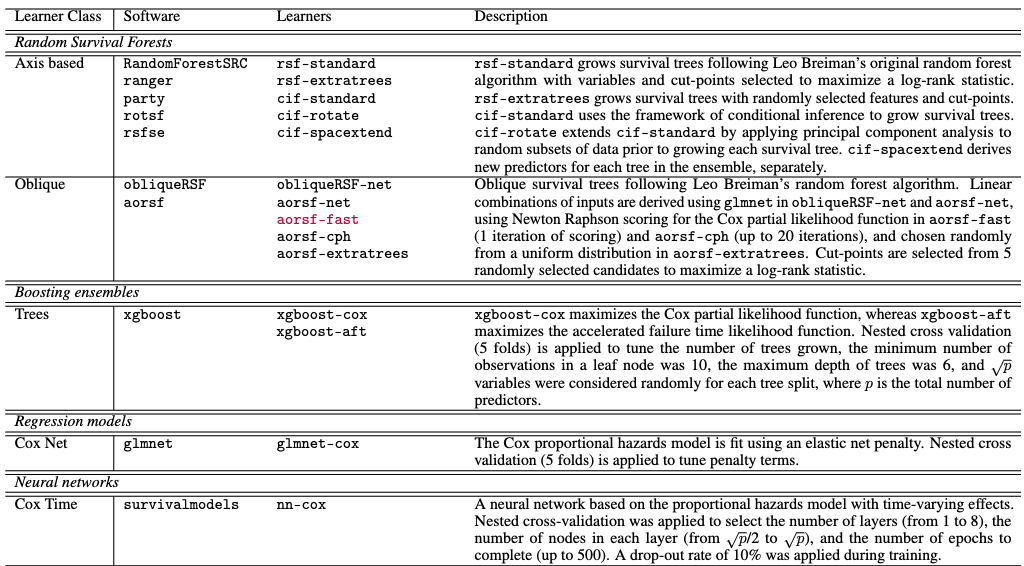
\includegraphics[scale=0.42]{Figures/OBLIQUE_SUMMARY.png}
    \caption{\parencite{jaeger_accelerated_2022} Shows available packages based on model types for random survival forests.}
\end{figure}

\subsection{Applied example of these models in a simulation studies}

\noindent \parencite{kurt_omurlu_comparisons_2009} Evaluated and compared the effectiveness of Cox regression analysis (CRA) and random survival forests (RSF) through both simulated and actual breast cancer data scenarios. Initially, the study utilized Monte Carlo simulations to assess how both methods performed across various sample sizes, specifically observing their performance metrics based on Harrell's concordance index. The results indicated that CRA consistently outperformed RSF under simulation conditions, particularly when using the concordance index for evaluation. Following the simulations, the methods were applied to a real dataset comprising 279 breast cancer patients to identify major risk factors influencing disease-free survival (DFS). In this practical application, RSF slightly edged out other methods, offering marginally better performance according to the concordance index when using the approximate log-rank splitting rule, compared to the other log-rank rules.
\\\\
\noindent \parencite{kurt_omurlu_comparisons_2009} CRA was noted for its predictive accuracy across different sample sizes, making it suitable for a broad range of survival data applications. Conversely, RSF was recommended for its interpretative power, especially beneficial in handling complex datasets where multiple survival trees are analyzed.
\\\\
\par \noindent Furthermore, \parencite{kantidakis_simulation_2021} shows a comparison between a machine learning method, termed survival neural networks (SNNs) and compared it with the Cox proportional hazards model, using clinical trial data for survival outcomes. The models are formulated subject to the European Osteosarcoma intergroup trial data, which is used as the foundation for the synthetic data generation that would ultimately be used for simulation training. The original dataset contains various instances of censoring, and the authors approach this issue, by segmenting the datasets into samples with degrees of censoring present (20\%, 40\%, 61\%, 80\%), after which data imputation techniques such as the inverse probability weighting, censoring method (IPW), was used, which is based on calibration procedures outlined in the paper, to ensure the synthetic data retains the statistical properties of the original clinical data. 
\\\\
\noindent Accuracy (Brier) interpreted in continuous form as the integrated Brier score for prediction error over the total period, and lastly Miscalibration (mean squared error) for censored groups. \parencite{kantidakis_simulation_2021} The results indicated comparable predictive performance but highlighted a lack of accuracy for calibration measures with SNNs. The authors point out that although machine learning techniques are attractive for survival analysis scenarios because of the ability to model interactions and nonlinearities with a no-assumption approach, the robustness of the Cox model, regarding ease of implementation as well as interpretability of covariates makes it formidable in situations where limited sample sizes and variables are available. The paper ties in nicely with the other literature in support of the need for clear and better implementation of calibration metrics specifically with machine learning models, and caution against indiscriminate application of these models.

\section{Data Generating Mechanisms For Simulation}
\noindent Methods for extrapolating missing data, speaks to the key feature of survival analysis and the difficult problem of dealing with censored data. Several different methodologies and considerations exist outlining how to impute, simulate, and generate data, for different settings of survival data.

\subsection{Data Simulation Methods}
\noindent \parencite{thurow_how_2023} Shows that there is a scarcity of publicly available real-world datasets for benchmarking models in oncology, particularly those that comply with the FAIR Data Principles. This significantly limits the ability to conduct model comparisons using real patient data, which is crucial for ensuring the models' applicability and robustness in real-world scenarios. The challenge of simulating realistic survival data for model comparison in situations where real-world data is not available or is incomplete. This is particularly relevant for ensuring that simulated data can reliably mimic real-world outcomes to validate model performance effectively. \parencite{thurow_how_2023} proposes several methods for dealing with data simulation.
\begin{figure}
    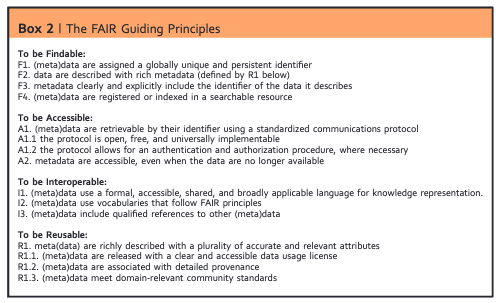
\includegraphics[scale=0.85]{Figures/FAIR_PRINCIPLES.png}
    \caption{\parencite{wilkinson_fair_2016} Fair principles summary}
\end{figure}

\subsection{Data Imputation Methods} \label{impute}
Data imputation is crucial for addressing issues arising from censored data by replacing missing values with values that resemble others in the distribution. Censoring happens because of factors like; the end of the observation period, loss before observation, or discontinuation of study participation. This often prevents the collection of complete data on the time until an event of interest occurs and so \parencite{jin_imputation_2024} classifies these scenarios into censoring classes; censored at random as well as censored not at random (CAR \& CNAR). Data imputation is relevant to these contexts to correct for the potential biases introduced by censoring, especially when it is informative or non-random. \parencite{jin_imputation_2024} Shows the Cox Proportional Hazards model assumes noninformative censoring (CAR) for its analysis. In cases where this assumption might not hold due to practical reasons, such as decisions influenced by patient or physician preferences, they point to data imputation under CNAR assumptions as a way to account for potential biases. Under the CAR assumption \parencite{jin_imputation_2024}, the hazard function after censoring is assumed to be the same as if the subject had not been censored, conditional on the covariates. This reflects the assumption that the censoring is non-informative regarding the survival probability. This means that the survival and hazard functions do not need special adjustments beyond the point of censoring other than ensuring that the analysis correctly accounts for the time of censoring. For CNAR, \parencite{jin_imputation_2024} the assumption is that the hazard of having an event after censoring may differ from that before censoring due to the censoring being potentially dependent on unobserved variables affecting the hazard. Mathematically, this means the post-censoring hazard function cannot simply extend the pre-censoring model. In practical terms, the CNAR model needs to be specifically formulated to reflect how the hazard might increase or decrease post-censoring due to factors related to why the censoring occurred. This could involve modifying the functional form of \(\lambda_{post}\) or using additional data and techniques to estimate it. \parencite{jin_imputation_2024} Shows 4 methods for handling data imputation under the CNAR and CAR assumptions.

\subsection{Synthetic Data Generation Methods}
Machine learning methods for simulation and data generation have risen in popularity recently, \parencite{norcliffe_survivalgan_2023} shows multiple methods combining statistical imputation methods into machine learning architectures. Specifically \parencite{norcliffe_survivalgan_2023} extend prior work for survival analysis to generate synthetic data using a Conditional Generative Adversarial Network (GAN) framework. The process integrates various components to handle different data types and ensure a realistic simulation of survival times based on censoring and event data.

\begin{figure}[h]
    \centering
    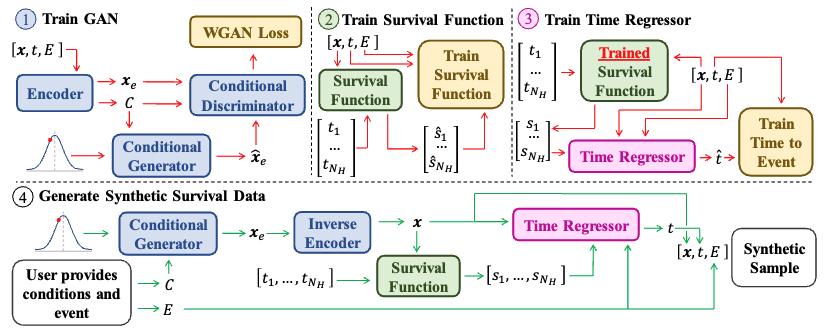
\includegraphics[scale=0.49]{Figures/GAN_ARCH.png}
    \caption{\parencite{norcliffe_survivalgan_2023} Survival GAN architecture}
\end{figure}
\pagebreak

\noindent The tabular encoder converts continuous features into a format suitable for the GAN using a Gaussian Mixture Model (GMM) \parencite{norcliffe_survivalgan_2023}; each feature is represented by its GMM component and deviation from the component mean. Categorical features are directly converted into one-hot vectors. The Encoder simplifies the full tabular encoding to just the one-hot vector component, representing condition C for the generator. For the Survival GAN architecture, they used models like DeepHit \parencite{norcliffe_survivalgan_2023} to estimate probabilities. The Time Regressor component predicts the actual time of an event or censoring based on the outputs of the survival function and the event type (E). This component can utilize various regression models, such as XGBoost \parencite{norcliffe_survivalgan_2023}.
\\\\
\noindent During training the loss function used was a Wasserstein GAN \parencite{norcliffe_survivalgan_2023} with a gradient penalty which ensures stable training of the GAN by adjusting the generator and discriminator losses to minimize the distance between real and generated data distributions while penalizing gradient norms. This allows for user-defined or sampled conditions and events. The GAN uses these to generate encoded covariates, which are then decoded back to their original form. These covariates are input into the survival function and time regressor to finally produce the synthetic time-to-event data. This architecture allows SurvivalGAN to realistically model survival data by accurately simulating the underlying time-to-event dynamics and handling various data imbalances and types.

\begin{figure}[h]
    \centering
    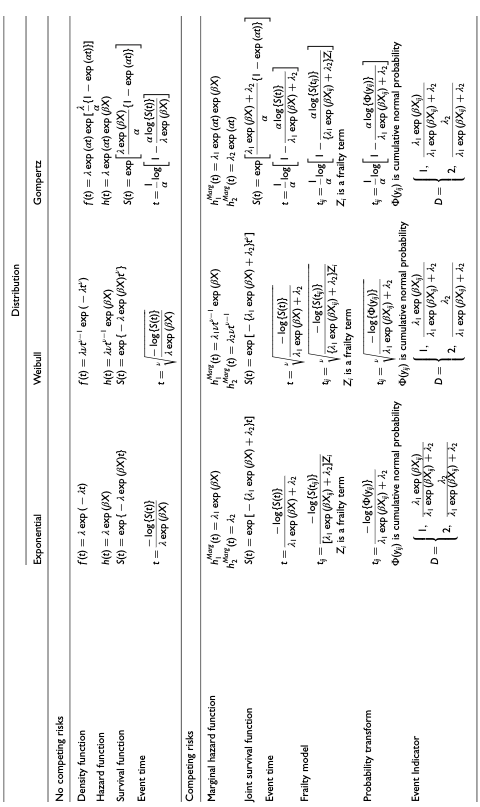
\includegraphics[scale=0.56 , angle=270]{Figures/COMPETING1.png}
    \caption{\parencite{meng_simulating_2023} Shows simulation formulas under spesific conditions.}
\end{figure}
\section{Model Evaluation And Result Interpretation} \label{eval}
In evaluating the performance of survival prediction models, it is crucial to employ metrics that not only assess accuracy but also ensure fairness by minimizing bias. This involves selecting evaluation measures that effectively balance calibration (the agreement between predicted and observed outcomes) and discrimination (the model's ability to distinguish between different outcomes). \parencite{sonabend_flexible_2022} Provides a guidelines and comprehensive framework for assessing model performance against true event times, ensuring that the models are both fair and accurate across different scenarios. These are essential for advancing survival analysis in ethically sensitive domains, thereby supporting more reliable and equitable outcomes. Following are some common methods to evaluate model results.

\subsection{C-Index}
\noindent Variants of the C-index include; the time-independent C-index (Cti) which negates survival probability at some specified period. It assesses the sequence of actual event times matches the predicted times, time-dependent C-index (Ctd) shown by \parencite{qi_effective_2023} and it accounts for varying amounts of censoring over time. The C-index can be biased upwards with a high level of censoring in the data. This issue is addressed through the Ctd rule, although it is not a proper scoring rule \parencite{qi_effective_2023}. The C-index, while useful, does not always align with other metrics such as the Mean Absolute Error (MAE). A model can have a high C-index (accurately ranking the order of events) while still having large discrepancies in the actual predicted times of those events.

\subsection{Brier Score and Integrated Brier Score}
The Brier Score and the Integrated Brier score (IBS) are essential metrics used to evaluate the accuracy and reliability of survival models \parencite{haider_effective_2018}. Both scores measure the calibration and discrimination capabilities of a model, which are crucial for producing unbiased and precise predictions in survival analysis. Below is a detailed explanation of both metrics. A perfect model, which perfectly predicts whether events happen by time \(t^{*}\) (predicting 1s and 0s accurately), would have a Brier score of 0. A model that always predicts a 50\% chance of survival regardless of the actual outcome will have a Brier score of 0.25, representing poor predictive accuracy. IBS is particularly useful for survival prediction models where it is important to assess model performance comprehensively across time rather than at a single time point. It gives an average score that reflects the overall performance of the model across the specified time interval. For censored data, the Inverse Probability Censoring Weight (IPCW) \parencite{haider_effective_2018} technique is often used in conjunction with IBS to adjust the contributions of censored subjects. This method helps to ensure that the model's performance is not unduly biased by the censoring. IBS is considered a proper scoring rule if the censoring distribution is estimated correctly, meaning it incentivizes truthful forecasting and accurately reflects the model's predictive capabilities. IBS can be particularly impactful in clinical settings where decisions might depend on accurate, time-specific survival probabilities, such as deciding on conservative treatments based on predicted long-term survival chances.

\subsection{Hosmer-Lemeshow Calibration (1-Calibration)}
1-Calibration \parencite{haider_effective_2018} measures how well the predicted probabilities of an event (e.g., failure, death) occurring by \(t^{*}\) match the actual proportion of those events in the dataset. This test is particularly useful in contexts where predictions need to be reliable at specific critical thresholds. A low value of the Hosmer-Lemeshow statistic \parencite{qi_effective_2023} suggests that the model's predictions are well-calibrated i.e. the predicted probabilities of survival match the actual rates observed. The statistic follows a chi-squared distribution \parencite{qi_effective_2023}, allowing for the derivation of a p-value to assess the significance of the results. A model is considered well-calibrated at the chosen significance level if the p-value is greater than 0.05.

\subsection{D-Calibration}
D-Calibration measures the consistency of predicted probabilities across a range of outcomes within a dataset. It assesses whether the distribution of predicted probabilities (over time or across conditions) matches the observed distribution of outcomes \parencite{haider_effective_2018}. Predicted probabilities are checked across a range of values. For each interval [a,b] within the probability range [0,1], the proportion of subjects with predicted probabilities within this range is compared to the actual proportion of events occurring in this interval. The fraction of subjects per interval is expected to match the width of the interval \(b-a\). For instance, for the interval [0.1, 0.2], approximately 10\% of the subjects should ideally have their predicted probabilities fall within this range if the model is perfectly D-Calibrated \parencite{haider_effective_2018}. A chi-squared test can be used to assess the uniformity of the distribution of predictions across the intervals, providing a statistical measure of calibration \parencite{haider_effective_2018}.

\subsection{Scoring Theory}
\par \noindent Scoring rules are essential tools in statistics and machine learning for evaluating the accuracy of probabilistic predictions. \parencite{yanagisawa_proper_2023} It is used to measure the quality of predictions by assigning a numerical score based on the probability forecast and the actual outcome. Thus it helps assess how well a model predicts the timing of future events, such as failures or deaths. A proper scoring rule incentivizes truthful forecasting \parencite{yanagisawa_proper_2023}, meaning it rewards the forecaster if the predicted distribution closely matches the true distribution of outcomes. A scoring rule is called proper \parencite{yanagisawa_proper_2023} if the expected score is minimized when the prediction model uses the true probability distribution. It is strictly proper if the score is uniquely minimized by the true distribution \parencite{yanagisawa_proper_2023}.

\noindent Proper Scoring Rule:
\begin{equation} \label{eq:proper}
E[(t,c) \sim (T,C)][S(\hat{F}, (z, \delta))] \geq E[(t,c) \sim (T,C)][S(F, (z, \delta))]
\end{equation}

\noindent Strictly Proper Scoring Rule:
\begin{equation} \label{eq:strictproper}
E[(t,c) \sim (T,C)][S(\hat{F}, (z, \delta))] > E[(t,c) \sim (T,C)][S(F, (z, \delta))] \quad \text{if} \quad \hat{F} \neq F
\end{equation}
